\documentclass[a4paper]{article}
\usepackage{amsmath}
\usepackage{amsfonts}
\usepackage{amssymb}
\usepackage{graphicx}
\usepackage{float}

\begin{document}

\noindent \large Auteur: Siebe Haché \\
\noindent \large Studierichting: Informatica \\
\noindent \large Oefeningenreeks 5M nr. 2 \\

\medskip
\normalsize

Bereken de oppervlakte $S$ van het lichaam dat men krijgt door de astroïde met parametervoorstelling $\begin{cases} x(t) = a \cos^3 t \\ y(t) = a \sin^3 t \end{cases}$ te wentelen rond de $x$-as. \\

afgeleiden: \\

$x'(t) = 3a \cos^2t (-\sin t) = -3a \cos^2t \sin t$ \\

$y'(t) = 3a \sin^2t (\cos t) = 3a\sin^2t \cos t$ \\

wortel: \\

$\sqrt{(x'(t))^2 + (y'(t))^2} = \sqrt{(-3a \cos^2 t \sin t)^2 + (3a \sin^2 t \cos t)^2}$\\

$= \sqrt{9a^2 \cos^4t \sin^2t + 9a^2 \sin^4t \cos^2t}$ \\

$= \sqrt{9a^2\cos^2t \sin^2t (\cos^2 t + \sin^2 t)}$\\

$= \sqrt{9a^2\cos^2t \sin^2t (1)} = 3a |\cos t \sin t|$ \\

Integraal:\\

$S = 4\pi \displaystyle\int_{0}^{\dfrac{\pi}{2}} (a \sin^3 t) (3a \cos t \sin t)dt$ \\

$= 12\pi a^2 \displaystyle\int_{0}^{\dfrac{\pi}{2}} \sin^4 t \cos t dt$\\

Stel $u = \sin t$, $du = \cos t dt$\\

$S = 12\pi a^2 \displaystyle\int_{0}^{1} u^4 du$\\

$= 12\pi a^2 \left[ \dfrac{u^5}{5} \right]_{0}^{1}$\\

$= 12\pi a^2 \left( \dfrac{1}{5} - 0 \right) = \dfrac{12\pi a^2}{5}$ \\



\begin{figure}[H]
 \centering
 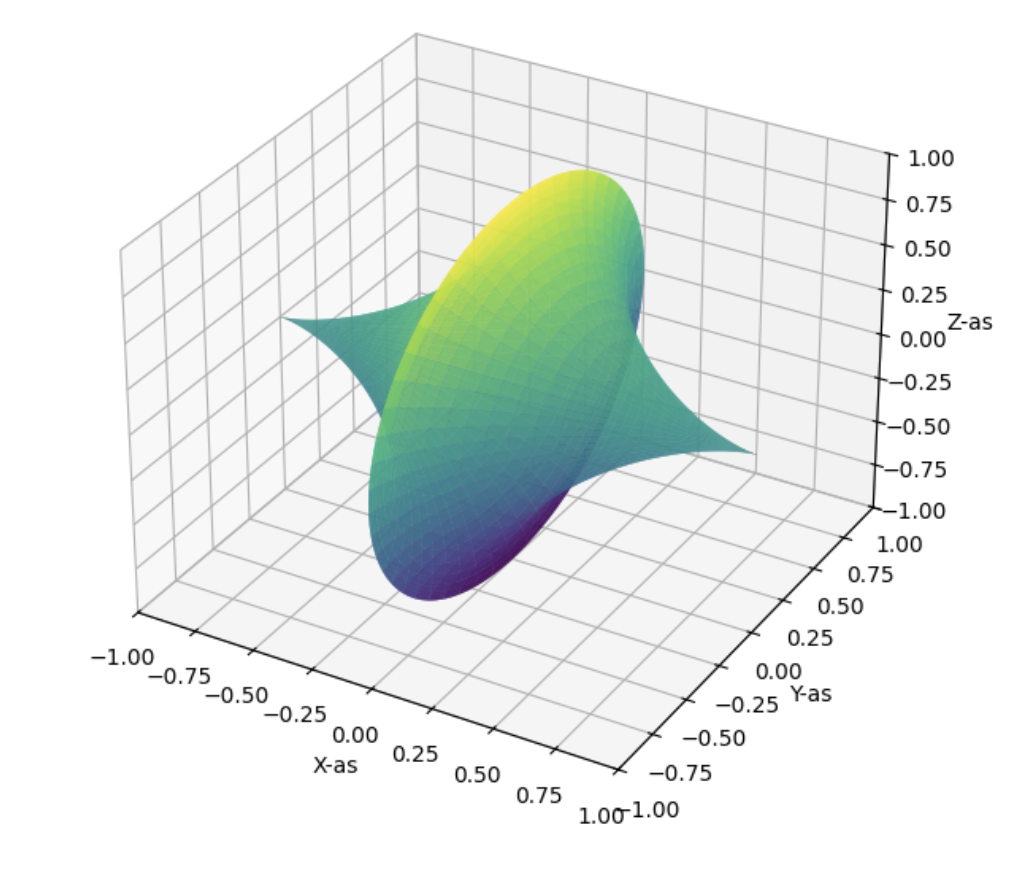
\includegraphics[width=0.6\textwidth]{5M-2-siebe.hache.INF.png}
\end{figure}

\begin{thebibliography}{999}
\bibitem{a} Grafiek gemaakt met Python
\end{thebibliography}

\end{document}